\subsubsection{Use Case Diagramm}
\begin{figure}[hp]
	\centering
		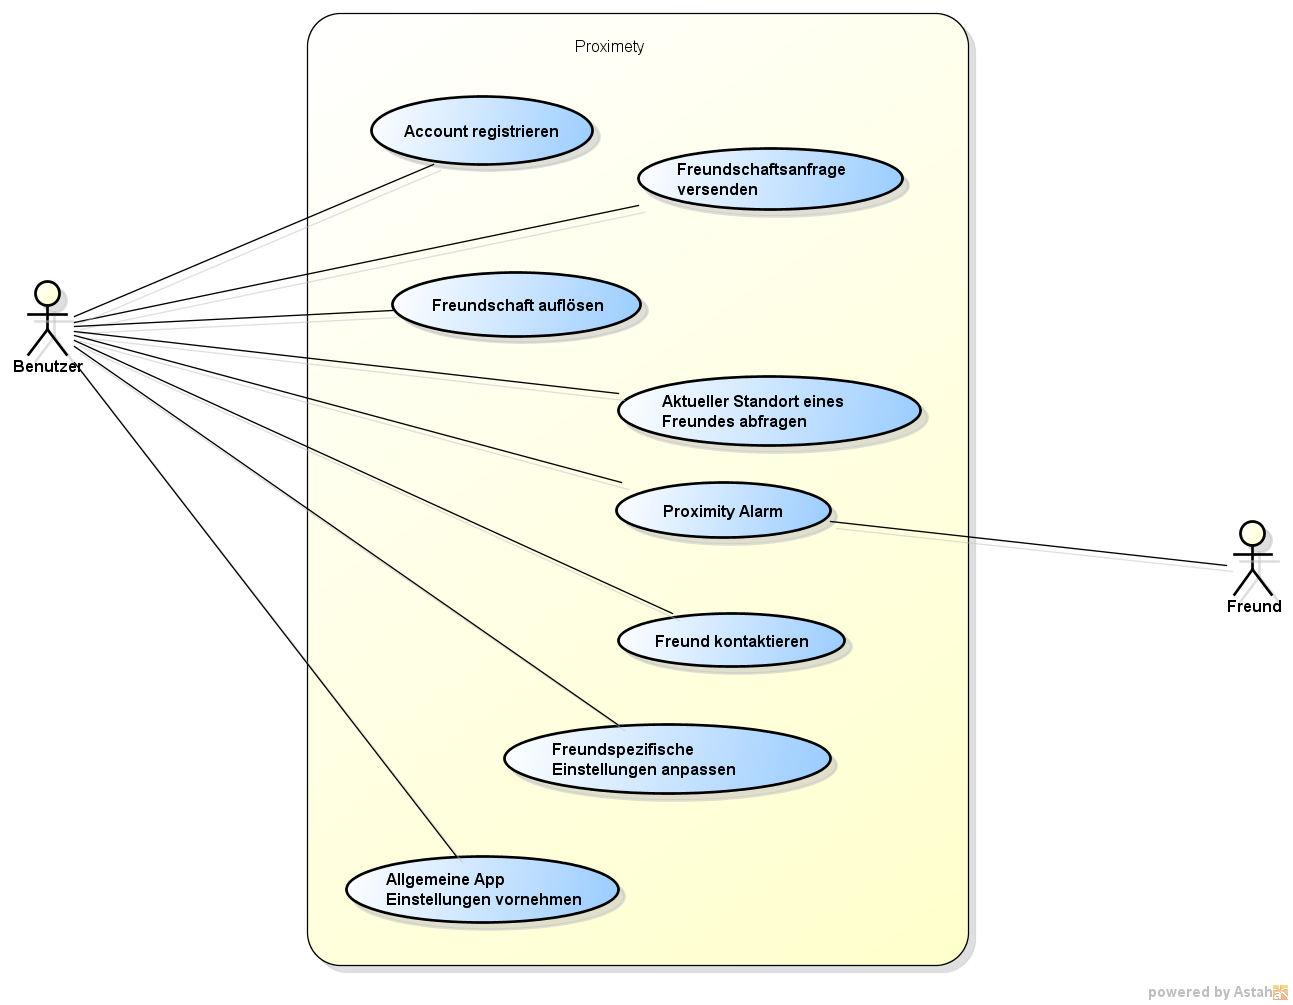
\includegraphics[scale=0.4]{BasicUseCaseDiagramm.png}
	\caption{Basis UseCase Diagramm}
	\label{fig:BasicUseCaseDiagramm}
\end{figure}
\FloatBarrier
% ------------------------------------------------------------------
\subsubsection{Use Case Beschreibungen}
% ------------------------------------------------------------------
\paragraph{UC01 - Account registrieren}
\begin{usecase}	
	\ucElement{ID}{UC01}
	\ucElement{Name}{Account registrieren}
	\ucElement{Kurzbeschreibung}{Der Benutzer registriert sich am System und erhält Logindaten.}
	\ucElement{Akteur}{Benutzer}
	\ucElement{Auslöser}{Der Akteur beginnt mit der Registrierung}
	\ucElement{Vorbedingungen}{App muss auf dem Gerät des Benutzers}
	\ucElement{Eingehende Informationen}{E-Mailadresse, Benutzername, Passwort}
	\ucElement{Ergebnis}{Registrierungsbestätigung}
	\ucElement{Nachbedingungen}{Benutzerkonto wurde erstellt}
	\ucElement{Ablauf}{%
		\begin{enumerate}
			\item Akteur startet Registrierungsprozess
			\item Akteur gibt E-Mailadresse und Passwort ein (inkl. Bestätigung)
			\item Akteur gibt Benutzernamen ein
			\item Akteur bestätigt die Registrierung.
		\end{enumerate}
		Es wird explizit darauf verzichtet eine aktivierungs E-Mail zu versenden.     
	}
	\ucElement{Alternativer Ablauf}{ %
				\begin{enumerate}
					\item[4a.]  Benutzername oder E-Mail werden bereits verwendet. Benutzer wird aufgefordert diese zu ändern.
				\end{enumerate}
		}
	\ucElement{Priorität}{Hoch}
	\ucElement{Aufwand}{?}
	\ucElement{Status}{Offen}
	\ucElement{Änderungshistorie}{?}
\end{usecase}
% ------------------------------------------------------------------
\paragraph{UC02 - Freundschaftsanfrage versenden}
\begin{usecase}	
	\ucElement{ID}{UC02}
	\ucElement{Name}{Freundschaftsanfrage versenden}
	\ucElement{Kurzbeschreibung}{Der Benutzer sendet eine Anfrage an einen anderen Benutzer um ihn seiner persönlichen Freundesliste hinzu zufügen.}
	\ucElement{Akteur}{Benutzer}
	\ucElement{Auslöser}{Der Akteur beginnt mit der Suche nach einem Freund}
	\ucElement{Vorbedingungen}{Benutzer besitzt einen Account}
	\ucElement{Eingehende Informationen}{E-Mailadresse oder Benutzername eines Benutzers}
	\ucElement{Ergebnis}{Freundesanfrage an anderen Benutzer}
	\ucElement{Nachbedingungen}{}
	\ucElement{Ablauf}{%
		\begin{enumerate}
			\item Akteur sucht einen Benutzer anhand Benutzername oder E-Mail
			\item Akteur wählt Benutzer aus Ergebnisliste aus um eine Anfrage zu versenden
			\item Angefragter Benutzer entscheidet über die Anfrage (Annahme/Ablehnen)
			\item Akteur wird über das Ergebnis informiert.
		\end{enumerate}    
	}
	\ucElement{Alternativer Ablauf}{}
	\ucElement{Priorität}{Hoch}
	\ucElement{Aufwand}{?}
	\ucElement{Status}{Offen}
	\ucElement{Änderungshistorie}{?}
\end{usecase}
% ------------------------------------------------------------------
\paragraph{UC03 - Freundschaft auflösen}
\begin{usecase}	
	\ucElement{ID}{UC03}
	\ucElement{Name}{Freundschaft auflösen}
	\ucElement{Kurzbeschreibung}{Der Benutzer entfernt einen anderen Benutzer von seiner Freundesliste}
	\ucElement{Akteur}{Benutzer}
	\ucElement{Auslöser}{Der Akteur möchte einen Freund aus seiner Liste entfernen.}
	\ucElement{Vorbedingungen}{ %
		\begin{itemize}
			\item Benutzer besitzt einen Account
			\item Benutzer besitzt mind. einen Freund			
		\end{itemize}
		}
	\ucElement{Eingehende Informationen}{Der zu entfernende Freund}
	\ucElement{Ergebnis}{Benachrichtigung an beide Benutzer}
	\ucElement{Nachbedingungen}{Akteur und ausgewählter Benutzer sind keine Freunde mehr.}
	\ucElement{Ablauf}{%
		\begin{enumerate}
			\item Akteur sucht einen Benutzer in seiner Freundesliste			
			\item Akteur wählt Benutzer aus und wählt “Freund entfernen”
			\item Akteur bestätigt seine Wahl (Annahme/Ablehnen)
			\item Beide Benutzer werden über das Ereignis informiert
		\end{enumerate}    
	}
	\ucElement{Alternativer Ablauf}{}
	\ucElement{Priorität}{Mittel}
	\ucElement{Aufwand}{?}
	\ucElement{Status}{Offen}
	\ucElement{Änderungshistorie}{?}	
\end{usecase}
% ------------------------------------------------------------------
\paragraph{UC04 - Aktueller Standort eines Freundes abfragen}
\begin{usecase}	
	\ucElement{ID}{UC04}
	\ucElement{Name}{Aktueller Standort eines Freundes abfragen}
	\ucElement{Kurzbeschreibung}{Der Benutzer fragt den aktuellen Standort eines Freundes ab. Dieser wird auf einer Karte angezeigt}
	\ucElement{Akteur}{Benutzer}
	\ucElement{Auslöser}{Der Akteur möchte einen Freund lokalisieren.}
	\ucElement{Vorbedingungen}{ %
		\begin{itemize}
			\item Benutzer besitzt einen Account
			\item Benutzer besitzt mind. einen Freund			
		\end{itemize}
	}
	\ucElement{Eingehende Informationen}{Der zu lokalisierende Freund}
	\ucElement{Ergebnis}{Standort des Freundes}
	\ucElement{Nachbedingungen}{}
	\ucElement{Ablauf}{%
		\begin{enumerate}
			\item Akteur sucht einen Benutzer in seiner Freundesliste			
			\item Akteur wählt Benutzer aus und wählt “Freund lokalisieren”
			\item Aktueller Standort wird von Freund abgerufen und auf einer Karte dargestellt.
		\end{enumerate}    
	}
	\ucElement{Alternativer Ablauf}{ %
		\begin{enumerate}
			\item[3a.] Standort kann nicht abgerufen werden: Entsprechende Fehlermeldung wird angezeigt. 
		\end{enumerate}
		}
	\ucElement{Priorität}{Hoch}
	\ucElement{Aufwand}{?}
	\ucElement{Status}{Offen}
	\ucElement{Änderungshistorie}{?}
\end{usecase}
% ------------------------------------------------------------------
\paragraph{UC05 - Proximity Alarm}
\begin{usecase}	
	\ucElement{ID}{UC05}
	\ucElement{Name}{Proximity Alarm}
	\ucElement{Kurzbeschreibung}{Benachrichtigung falls sich zwei Benutzer in definierter (oder weniger) Distanz zueinander befinden.}
	\ucElement{Akteur}{System}
	\ucElement{Auslöser}{System ermittelt Distanz zwischen Benutzern unter definiertem Schwellwert.}
	\ucElement{Vorbedingungen}{ %
		\begin{itemize}
			\item Beide Benutzer sind Freunde
			\item Aktueller Standort von beiden Benutzern bekannt
			\item Proximity Alarm für Freund aktiviert			
		\end{itemize}
	}
	\ucElement{Eingehende Informationen}{Standort der Benutzer}
	\ucElement{Ergebnis}{Benachrichtigung der beiden Benutzer}
	\ucElement{Nachbedingungen}{}
	\ucElement{Ablauf}{%
		\begin{enumerate}
			\item System prüft periodisch die Distanz zwischen Freunden			
			\item System versendet Benachrichtigung an die Benutzer
		\end{enumerate}    
	}
	\ucElement{Alternativer Ablauf}{}
	\ucElement{Priorität}{Hoch}
	\ucElement{Aufwand}{?}
	\ucElement{Status}{Offen}
	\ucElement{Änderungshistorie}{?}
\end{usecase}
% ------------------------------------------------------------------
\paragraph{UC06 - Freund kontaktieren}
\begin{usecase}	
	\ucElement{ID}{UC06}
	\ucElement{Name}{Freund kontaktieren}
	\ucElement{Kurzbeschreibung}{Benutzer kann einen Freund aus der App mit dritt Apps kontaktieren}
	\ucElement{Akteur}{Benutzer}
	\ucElement{Auslöser}{Benutzer möchte Freund kontaktieren}
	\ucElement{Vorbedingungen}{Beide Benutzer sind Freunde}
	\ucElement{Eingehende Informationen}{E-Mail des Freundes (z.Z. keine weiteren Kontaktinformationen vorhanden)}
	\ucElement{Ergebnis}{Dritt-App wird mit Kontaktinformationen (E-Mail) gestartet}
	\ucElement{Nachbedingungen}{}
	\ucElement{Ablauf}{%
		\begin{enumerate}
			\item Akteur sucht einen Benutzer in seiner Freundesliste			
			\item Benutzer wählt Kontakt App aus (z.B. Gmail)
			\item Dritt-App wird gestartet
		\end{enumerate}    
	}
	\ucElement{Alternativer Ablauf}{}
	\ucElement{Priorität}{Tief}
	\ucElement{Aufwand}{?}
	\ucElement{Status}{Offen}
	\ucElement{Änderungshistorie}{?}
\end{usecase}
% ------------------------------------------------------------------
\paragraph{UC07 - Freund-Spezifische Einstellungen anpassen}
\begin{usecase}	
\ucElement{ID}{UC07}
\ucElement{Name}{Freund-Spezifische Einstellungen anpassen}
\ucElement{Kurzbeschreibung}{Benutzer kann für jeden Freund Einstellungen anpassen (Tracking ein/aus, Distanz)}
\ucElement{Akteur}{Benutzer}
\ucElement{Auslöser}{Benutzer möchte Einstellungen ändern}
\ucElement{Vorbedingungen}{Beide Benutzer sind Freunde}
\ucElement{Eingehende Informationen}{Gewünschte Einstellungen}
\ucElement{Ergebnis}{Einstellungen sind angepasst}
\ucElement{Nachbedingungen}{}
\ucElement{Ablauf}{%
	\begin{enumerate}
		\item Akteur sucht einen Benutzer in seiner Freundesliste
		\item Benutzer ändert Einstellungen (Tracking ein/aus, Distanz)
		\item Benutzer bestätigt Eingaben
	\end{enumerate}       
}
\ucElement{Alternativer Ablauf}{}
\ucElement{Priorität}{Mittel}
\ucElement{Aufwand}{?}
\ucElement{Status}{Offen}
\ucElement{Änderungshistorie}{?}
\end{usecase}
% ------------------------------------------------------------------
\paragraph{UC08 - Allgemeine App Einstellungen vornehmen}
\begin{usecase}	
	\ucElement{ID}{UC08}
	\ucElement{Name}{Allgemeine App Einstellungen vornehmen}
	\ucElement{Kurzbeschreibung}{Der Benutzer kann allgemeine Einstellungen an der App vornehmen}
	\ucElement{Akteur}{Benutzer}
	\ucElement{Auslöser}{Der Akteur möchte Einstellungen ändern}
	\ucElement{Vorbedingungen}{ Benutzer besitzt einen Account}
	\ucElement{Eingehende Informationen}{}
	\ucElement{Ergebnis}{Einstellungen aktualisiert und gespeichert}
	\ucElement{Nachbedingungen}{}
	\ucElement{Ablauf}{%
		\begin{enumerate}
			\item Akteur wählt in der Naviagtion “Einstellungen” aus			
			\item Akteur kann Einstllungen anpassen (Standard Distanz für Alarm, Alarm Ton/Typ)
			\item Akteur bestätigt seine Einstellungen
		\end{enumerate}    
	}
	\ucElement{Alternativer Ablauf}{}
	\ucElement{Priorität}{Mittel}
	\ucElement{Aufwand}{?}
	\ucElement{Status}{Offen}
	\ucElement{Änderungshistorie}{?}
\end{usecase}